\levelB{Experiment on random data detection}
\label{sec:exprandom}

In the previous sections, it was observed that the higher the number of classes being considered during the creation of a file fragment classification model, the higher is the error rate of this model. In addition, the comparison of pairs of classes indicated that high entropy data structures may be responsible by some part of those errors.

Prior to conducting experiments to find the major cause of error, a list of conceivable error sources (E1 to E4) was elaborated:
\begin{enumerate}[itemindent=\parindent,label=\textbf{E\arabic*.}]
    \item For some data structure, the model cannot distinguish it from random data. This can happen if the pattern in the data is too complex, beyond the capabilities of the model. It may be the case that in practice no model can perform this distinction or, instead, this may be a limitation of this particular model only. This situation may occur in files that use compression or cryptography, or more generally, any file type with high entropy.

    \item Different file types using the same data structure. It is common to a given file type to employ different types of data structures. If two or more file types make use of the same data structure, the existence of that structure will then not be sufficient to differentiate those file types, as it may belong to anyone of them.
    The reverse, a file type that uses multiple kinds of data structures, does not constitute a problem as it simply results in extra work during the model training.

    \item Same file type with multiple extensions. If the same file type appears in the dataset with multiple extensions, ``JPG'' and ``JPEG'' for example, the model will not be able to predict which label is used in the validation dataset for a given instance, since this distinction exists in the labelling but not in the content.

    \item Files that contain other files. Some file types need to embed other files. If the inner file is categorized, even if the model finds an unmistakable pattern, it will not match the label, which will be the extension of the outer file. A ``PDF'' file, for example, can embed a ``JPG'' file. If the model predict ``JPG'' as the class of a portion of this file, it will no match the instance label on the dataset, which would be ``PDF''.
\end{enumerate}

The first error source, E1, is the focus of this section. In the file fragment classification task, it is expected that some portion of the classifications errors of a given model be caused by its inability to recognize patterns in the data, if the data has high entropy. In these situations, even humans may be unable to tell if a sample is valid or if it is random data.

The three last error sources listed above, E2 to E4, are not explored in this study. They are similar in nature, as the last two may be viewed as special cases of E2. This error source comes from the practice of using the extension of the file as the class to each of its parts. An analogy with speech recognition would be to label each syllable of a spoken word using the word as its label and then try to predict the whole word using only a syllable.

Unfortunately, for the file fragmentation task the potential labels for smaller parts may be less obvious than it is for speech recognition. The best case scenario would be if the neural network itself could choose the labelling. But evaluating those predicted labels using labels of its own choosing would introduce bias, as it could prefer to create only easy labels. Saying that all file types are composed of ``data'' is correct, but it is unhelpful.

\levelC{Objective}
The goal of this experiment is to measure how many fragments with recognizable patterns a given file type has.

\levelC{Hypothesis}
The goal of this experiment is to test the hypothesis that part of the errors of file fragment classification  can be explained by the existence of data that has no structure detectable by the model. Not all file types possess this kind of data, and on those that do, they should compose only a portion of the file.


\levelC{Models}
For each file type, a new model is trained to classify a fragment into two classes, random or not random. The stopping condition used is 4 epochs without improvement in validation accuracy.
The same sampling, input, and output details described in section \ref{sec:evalmodels} were used here. The model that gave best results in that section, identified as ``CLD'', was selected to be used.


\levelC{Dataset}
The dataset creation for a given file type follows almost the same procedure mentioned in the previous section, but instead of selecting two file types, it selects one file type and uses a random data generator for the other class.
When the model training finishes, if the validation accuracy is not above 90\% for a given file type, a new pass is initiated, to create a new model from scratch. But the new pass discards the samples from the file type dataset that are classified as random by the model trained in the previous pass. The process is repeated until the accuracy is above 90\%.

The final model can then used in the original dataset, giving a count of how many fragments are correctly identified as not random.

For the file types that present more than 10\% of fragments classified as random, a second procedure was performed, discarding this time the fragments classified as not random. The procedure is repeated until the validation accuracy is between 49\% and 51\%.

The model trained with this second procedure can be used to count how many fragments are classified as random in the original dataset.

\levelC{Results}
For some file types, training achieved an accuracy higher than 90\% on the first pass. These are the file types where a model should have no difficulty finding patterns. For the remaining file types, only one additional pass was necessary.

Figure \ref{fig:not_random} shows, for each file type, the percent of 512 byte fragments identified as not random, the percent of fragments identified as random, and the accuracy of each model (two models for each file type).

\noindent
\begin{figure*}[htb!]
\centering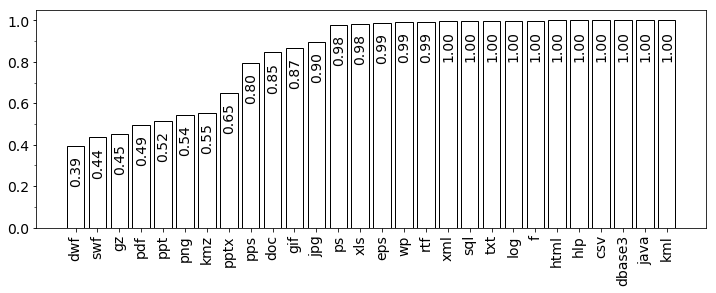
\includegraphics[width=0.50\textwidth]{content/random.png}
\caption{\label{fig:not_random}Validation accuracy of models trained to distinguish each file type from random data}%
\end{figure*}



\levelC{Limitations and threats to validity}
The procedure applied in this experiment avoids false positives over false negatives. In other words, it avoids random data classified as not random at the cost of missing potentially recognizable structures in valid fragments. Thus, it is expected that the exact valid fragments count, which is unknown in practice, will be higher than the number obtained.


% The extensions ``text'' and ``unk'' were also discarded because they do not correspond to a file type, and the files that use them belong to assorted types. 